
\section{Présentation du projet}
\label{sec:Présentation du projet}


    \subsection{sujet 4 :} le gardien de parc
		

\subsection{ Contexte}
\label{sec:spec1}
\paragraph{}L’intelligence artificielle est de plus en plus utilisée dans le monde d’aujourd’hui. Le
multi-agents réactifs est une méthode de programmation pour créer des intelligences artificielles.
Dans le cadre de notre formation à l’Université de Cergy Pontoise, les étudiants en Licence informatique deuxième année réalisent des projets personnels afin de valider leur année scolaire. Ce type de réalisation exige donc un certain temps, un investissement personnel et l’usage de toutes les ressources disponibles. Ici, nous allons réaliser notre projet sous la forme d’un jeu vidéo  appelé « le gardien de parc».

\subsection{ Objet}

\label{sec:spec2}
\paragraph{}Le but est la réalisation d’une application qui consiste à créer  un jeu qui permet de chasser les intrus  dans un espace  donné et de les éliminer.
  
\subsection{ Organisation}
\label{sec:spec3}
 \paragraph{}}Notre équipe est composée de trois membres à la charge du projet : Karabouali Makoura
, Phetramphand Antoine et Tangara Ramatoulaye. 
Pour mieux appréhender le projet, nous allons entamer des recherches et approfondir les non acquis et mettre le problème en œuvre techniquement en utilisant le processus «modèle en cascade». Il s'agit du modèle le plus simple des processus logiciels en termes de complexité et de facilité de mise en œuvre et repose sur les étapes suivantes :
		
		
\subsubsection{analyse}
\label{sec:spec1}
\paragraph{}On essaye de comprendre le problème ,puis d'analyser les besoins fonctionnels (contrainte technique).

\subsubsection{spécification}
\label{sec:spec2}
\paragraph{}On décrit les besoins du client, puis on traduit les besoins en fonctionnalités.

\subsubsection{conception}
\label{sec:spec3}
\paragraph{}On transforme le problème en solution.

\subsubsection{programmation}
\label{sec:spec4}
\paragraph{}On passe du résultat de la conception à un ensemble de programmes traduit en un langage de programmation ( Écriture des textes des programmes).

\subsubsection{tests}
\label{sec:spec5}
\paragraph{}On recherche des erreurs dans une spécification ou programme.

\subsubsection{validation}
\label{sec:spec6}
\paragraph{}Le système répond aux exigences du client et s'assure de l’adéquation des résultats de l'analyse et de la spécification.

\subsubsection{maintenance}
\label{sec:spec7}
\paragraph{}On veille au bon fonctionnement des programmes du projet.


\subsection{Environnement}
\label{sec:spec4}
\paragraph{}Les ressources  que nous disposons pour le développement de notre projet sont : 
\paragraph{Éclipse}:  un logiciel de développement. Son objectif est de produire et fournir des outils pour la réalisation de logiciels, englobant les activités de programmation permettant de réaliser notre projet en utilisant le langage Java.
\paragraph{SVN }: Subversion est un logiciel de gestion permettant de stocker , partager des fichiers texte informatique, et dispose d'un mécanisme intelligent de fusion des modifications apportées. C'est un outil très utilisé pour le développement de logiciels. 
\paragraph{Latex}: c'est un système de production de documents. Il ne s’agit pas de composer son texte, mais il s’agit d’utiliser un jeu de commandes décrivant ce que l’on souhaite obtenir.
 

\subsection{Plannification}
\label{sec:spec5}
\begin{figure}[h]
  \centering
  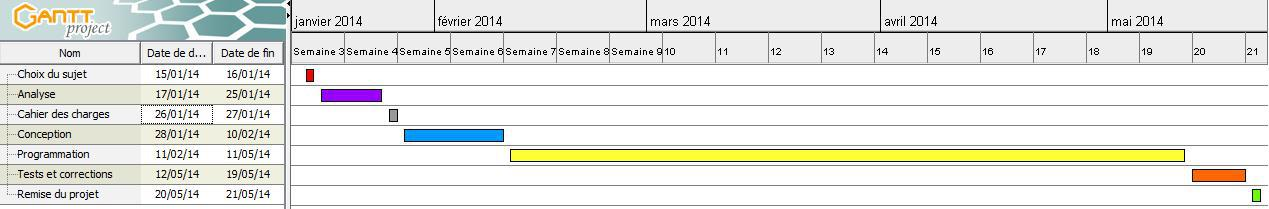
\includegraphics[width=500 , height=300]{images/planing.jpg}
  \caption{planning}
\end{figure}

